\documentclass{../content16b}
\usepackage[greek,  english]{babel}
% vanity commands
\let\conj\overline
\newcommand{\innerprod}[2]{%
  \ensuremath{\left\langle#1, #2\right\rangle}%
}
\newcommand{\transpose}[1]{\ensuremath{{#1}^\top}}
\DeclareMathOperator{\diag}{\mathrm{diag}}
\DeclareMathOperator{\proj}{\mathrm{proj}}
\DeclareMathOperator{\Span}{\mathrm{Span}}

\nouppercaseheads
\counterwithin{section}{chapter}
\aliaspagestyle{title}{empty}
\pagestyle{ruled}
%% not sure if I want to hang these!!
% \chapterstyle{hangnum}
% \hangsecnum


\newtheorem{infdef}{Informal Definition}
\newtheorem{definition}{Definition}
\newtheorem{lemma}{Lemma}
\newtheorem{theorem}{Theorem}

% \includeonly{lectures/27-lti, lectures/28-dft-convolution}
\begin{document}
\title{EECS 16B DFT Notes}
\renewcommand{\printchaptername}{\chapnamefont Lecture}

\tableofcontents

\chapter{The Discrete Fourier Transform}
\begin{flushright}
  O beloved son of Aegeus, for the gods alone\\
  there is no growing old, no dying ever.\\
  Everything else all-powerful Time destroys.\\
  (Sophocles, \emph{Oedipus at Colonus}, tr.~Lefkowitz and Romm)
  % Earth's strength fials, the body's strength fails,\\
  % trust dies, distrust blooms in its place\\
  % and the same spirit of friendliness never stays\\
  % between one man and anoth
\end{flushright}
The DFT basis uses the cyclic properties of the \(N\)th roots of unity to decompose a finite, discrete signal into periodic frequency components.

\section{Roots of 1}
\subsection{There are \(N\) of them}
What complex numbers \(\omega\) satisfy the equation \(\omega^N = 1\)?
Obviously 1 works.
To find the others, let \(\omega = re^{j\theta}\).
\begin{align}
  \del{re^{j\theta}}^N &= 1\\
  r^N e^{jN\theta} &= 1
  \intertext{Equating magnitudes, \(\left|r^N\right| = \left|r\right|^N = 1\).
  As \(r\) is a nonnegative real number, this means \(r = 1\).
  It can be cancelled from the left side.}
  e^{jN\theta} &= 1
  \intertext{This is satisfied when \(N\theta = 0\). As the complex exponential is periodic with a period of \(2\pi\), }
  N\theta &= 0, 2\pi, 4\pi, \ldots \\
  \theta &= 0, \frac{2\pi}{N}, \frac{4\pi}{N} \ldots \\
  \intertext{This list of options runs out of unique angles when \(\theta\) reaches \(2\pi\) again.
  Therefore, pairing each of these angles with magnitude \(r=1\), our solutions for \(\omega\) are}
  \omega &= e^{\frac{2\pi}{N}nj}, \quad n = 0, \ldots, N - 1.
\end{align}
These \(N\) numbers are called the \(N\)th roots of unity.
They can be viewed as the first \(N\) powers of \(e^{\frac{2\pi}{N}j}\), which is a rotation \(\frac{1}{N}\) of the way around the complex Unit Circle.
We will use the notation \(\omega_N = e^{\frac{2\pi}{N}j}\),\footnote{Any power \(\omega_N^r\), where \(r\) is prime to \(N\), will also generate all \(N\) roots of unity! This fact is amazing! Please ask me why in office hours!}
so that the \(N\)th roots of unity are \(\omega_N^0, \omega_N^1, \ldots, \omega_N^{N-1}\).

\subsection{They add to 0}
Because the \(N\)th roots of unity are all powers of \(\omega_N\), when you multiply them by \(\omega_N\), they don't go anywhere.
They just trade places.
We can use this coincidence to show that the sum of all the \(N\)th roots of unity is 0.

Call this sum \(S\).
We will multiply it by \(\omega_N\) and find that nothing changes.
\begin{align}
  S
  &= \sum_{n=0}^{N - 1}
  \omega_N^n\\
  \omega_N S
  &= \sum_{n=0}^{N - 1}
  \omega_N^{n+1}
  \intertext{The last term of this summation, \(\omega_N^N\), equals 1. Reordering the terms,}
  &= \sum_{n=0}^{N - 1}
  \omega_N ^n = S
\end{align}
We have shown that \(S\) is a number that you can multiply by a nonzero number and get \(S\) back.
Therefore \(S = 0\).

\subsection{They come in conjugate pairs}
Every \(N\)th root of unity comes with its complex conjugate:
if \(\omega^N = 1\), then \(\del{\overline \omega}^N = 1\).
This comes from conjugating the characterstic equation:
\begin{align}
  \omega^N &= 1\\
  \overline{\omega^N} &= \overline 1\\
  \del{\overline \omega}^{\overline N} &=
  \del{\overline \omega}^{N} = 1.
\end{align}

\section{The DFT Basis}
Define a basis \(\left\{u_0, \ldots, u_{N-1}\right\}\) for \(\mathbb{C}^N\) as follows:\footnote{Indexing from \(0\) presents this basis in the customary order.}
\begin{align*}
  u_{k}[n] &= \frac{1}{\sqrt{N}} \omega_N^{kn},
\end{align*}
where \(u_k[n]\) denotes the \(n\)th coordinate of basis vector \(u_k\).%
\footnote{Many normalizations of this basis exist. We are using the \(\frac{1}{\sqrt{N}}\) normalization because it's orthonormal, but it is not the most common default in numerical computing packages.}

\begin{theorem}[DFT is orthonormal]
  The DFT basis, defined above, is orthonormal.
\end{theorem}
\begin{proof}
  We need to check that \(\innerprod{u_k}{u_{k'}}\) equals 1 when \(k = k'\) and 0 otherwise.
  \begin{align}
    \innerprod{u_k}{u_{k'}}
    &= \sum_{n = 0}^{N - 1} u_k[n] \conj{u_{k'}[n]}\\
    &= \frac{1}{N}
    \sum_{n = 0}^{N - 1} \omega_N^{kn} \omega_N^{-k'n}\\
    &= \frac{1}{N}
    \sum_{n = 0}^{N - 1} \omega_N^{(k - k')n}
    \intertext{If \(k = k'\) then the sum is \(N\) and \(\innerprod{u_k}{u_{k'}} = 1\). Otherwise, write this sum using \(\zeta = \omega_N^{k - k'}\).}
    &= \frac{1}{N} \sum_{n = 0}^{N - 1} \zeta^n
  \end{align}
  This sum is stable  under multiplication by \(\zeta\), as \(\zeta^N = 1 = \zeta^0\), so it equals 0.
\end{proof}

By convention, in DFT contexts, indices start at zero and are interpreted modulo \(N\) because \(N\) roots of unity are \(N\)-cyclic; for example, the negative index \(-i\) can have the same meaning as the positive index \(N - i\).

The change of coordinates \emph{from} the DFT basis is called \textbf{synthesis} and is represented by \(F^* \in \mathbb{C}^{n \times n}\).
\begin{align}
  F^*_{kn} &= \frac{1}{\sqrt{N}} \omega_N^{kn}\\
  F^* &= \frac{1}{\sqrt N}\begin{pmatrix}
    1 & 1 & \ldots & 1\\
    1 & \omega & \ldots & \omega^{N - 1} \\
    1 & \vdots & \ddots & \vdots \\
    1 & \omega^{N- 1} & \hdots & \omega^{\del{N - 1}\del{N - 1}}
\end{pmatrix} & \text{(\textbf{synthesis matrix})}\\
x &= F^* X & \text{(\textbf{synthesis equation})}
\intertext{The change of coordinates \emph{to} the DFT basis is called \textbf{analysis} and is represented by \(F \in \mathbb{C}^{n \times n}\).}
F_{kn} &= \conj{F^*_{nk}} = \frac{1}{\sqrt{N}} \omega_N^{-kn}\\
F &= \frac{1}{\sqrt N}\begin{pmatrix}
  1 & 1 & \ldots & 1\\
  1 & \omega^{-1} & \ldots & \omega^{-\del{N - 1}} \\
  1 & \vdots & \ddots & \vdots \\
  1 & \omega^{-\del{N- 1}} & \hdots & \omega^{-\del{N - 1}\del{N - 1}}
\end{pmatrix}
& \text{(\textbf{analysis matrix})}\\
X &= F x & \text{(\textbf{analysis equation})}
\end{align}

``Synthesis'' and ``analysis'' are both words of Greek origin.
``Synthesis'' has the meaning of ``to put together,'' and ``analysis'' has the meaning of ``to take apart.''
\begin{itemize}
  \item If \(x\) records equally spaced samples of a signal, then DFT analysis is the process of shredding \(x\) into its frequency components \(X\).
  \item If \(X\) records the frequency components of \(x\), then DFT synthesis is the process of reassembling \(x\).
\end{itemize}
In the next section we will develop the interpretation of the DFT basis vectors as ``frequency components.''

\section{DFT of a sinusoid}
If the sinusoid \(\alpha\cos(\frac{2\pi k}{N}t + \varphi)\),
where \(k\) and \(N\) are integers,
is sampled \(N\) times in intervals of \(\Delta = 1\) starting at \(t = 0\),
the resulting sample vector is
\begin{align}
  x[n] &= \alpha\cos\del{\frac{2\pi k}{N}n + \varphi},
  \quad n = 0, \ldots, N - 1\\
  &= \frac{\alpha}{2}
  \del{e^{\del{\frac{2\pi k}{N}n + \varphi}j}
  + e^{-\del{\frac{2\pi k}{N}n + \varphi}j}}\\
  &= \frac{\alpha}{2}
  \del{e^{\frac{2\pi k}{N}nj} e^{\varphi j}
  + e^{-\frac{2\pi k}{N}nj} e^{-\varphi j}
  }\\
  &= \frac{\alpha}{2}
  \del{\del{e^{\frac{2\pi}{N}j}}^{kn} e^{\varphi j}
  + \del{e^{\frac{2\pi}{N}j}}^{-kn} e^{-\varphi j}
  }\\
  &= \frac{\alpha}{2}
  \del{\omega_N^{kn} e^{\varphi j}
  + \omega_N^{-kn} e^{-\varphi j}
  }\\
  &=
  \frac{\alpha}{2} e^{\varphi j} \omega_N^{kn}
  +
  \frac{\alpha}{2} e^{-\varphi j} \omega_N^{-kn}
  \\
  &=
  \frac{\alpha \sqrt N}{2} e^{\varphi j} u_k[n]
  +
  \frac{\alpha \sqrt N}{2} e^{-\varphi j} u_{N - k}[n]
  \\
  \intertext{In vector form,}
  x &=
  \frac{\alpha \sqrt N}{2} e^{\varphi j} u_k
  +
  \frac{\alpha \sqrt N}{2} e^{-\varphi j} u_{N - k}.
  \intertext{
  This expresses \(x\) as a superposition of \(u_k\) and \(u_{N -k}\).
  If \(k = 0\) modulo \(N\), then \(u_k = u_0 = u_{N - k}\) and \(x = \del{{\alpha \sqrt N} \cos{\varphi}} u_0\).
  If \(k \neq 0\) modulo \(N\), then  the Discrete Fourier Transform of \(x\) is the following:}
  X[n]
  &= \begin{cases}
    \frac{\alpha \sqrt N}{2} e^{\varphi j}, &n = k\\
    \frac{\alpha \sqrt N}{2} e^{-\varphi j}, &n = N - k\\
    0, & \text{else}
  \end{cases}
\end{align}
Note the following:
\begin{itemize}
  \item \(x\) is full of samples, but \(X\) is mostly zero.
  \item \(u_k\) and  \(u_{N - k}\) are conjugate, and so are their coefficients in \(x\).
  \item The DFT can extract a ``phasor representation'' of a sampled sinusoid.
  \item (The DFT can't tell the difference between \(k\) and \(k + N\).)
\end{itemize}

\chapter{DFT of a square wave}
% Last lecture we showed that
% if \(x \in \mathbb{C}^{N}\) is the following sinusoid sample:
% \begin{align}
%   x[n] &= \alpha\cos\del{\frac{2\pi k}{N}n + \varphi},
%   \quad n = 0, \ldots, N - 1
%   \intertext{Then its DFT is \(X \in \mathbb{C}^N\):}
%   X[n]
%   &= \begin{cases}
%     \frac{\alpha \sqrt N}{2} \cos{\varphi}, &n = k =0\\
%     \frac{\alpha \sqrt N}{2} e^{\varphi j}, &n = k \neq 0\\
%     \frac{\alpha \sqrt N}{2} e^{-\varphi j}, &n = N - k \neq N\\
%     0, & \text{else}
%   \end{cases}
% \end{align}
\section{Properties of the DFT}
In this section, let \(x\) and \(y\) be time domain signals of length \(N\) and \(X = Fx\) and \(Y = Fx\) be their DFTs.
\begin{itemize}
  \item The DFT is linear: if \(a\) and \(b\) are scalars, \(F(ax + by) = aFx + bFy\).
  \item The DFT preserves energy: \(\left\|Fx\right\|^2 = \left\|x\right\|^2\).
  \footnote{This is called Parseval's Theorem.}
  \item The DFT is conjugate-symmetric for real signals: if \(x\) is real, then \(X[n] = \conj{X[-n]} = \conj{X[N - n]} \).
\end{itemize}

\section{DFT of a rectangular pulse}
Let \(x \in \mathbb{C}^N\) be the following rectangular pulse, which approximates a square wave when \(M = N/4\):
\begin{align}
  x[n] &= \begin{cases}
    1, & -M \leq n \leq M\\
    0, & \text{else}
\end{cases}
\intertext{Then the DFT of \(x\) is given by the following analysis equation:}
  X &= Fx
\intertext{This can be expanded in terms of the columns of \(F\):}
  &= \sum_{k=-M}^M \conj{u_k}\\
  X[n]
  &= \sum_{k=-M}^M \conj{u_k[n]}\\
  &=
  \frac{1}{\sqrt{N}}
  \sum_{k=-M}^M \omega^{-kn} \\
  &=
  \frac{1}{\sqrt{N}}
  \sum_{k=-M}^M \del{\omega^{n}}^k \\
  \intertext{Use a formula for a finite geometric sum where the ratio is \(\omega^n\).}
  &=
  \del{\frac{1}{\sqrt{N}}}
  \frac{\del{\omega^n}^{-M} - \del{\omega^n}^{M + 1}}{1 - \omega^n}\\
  \intertext{Write each term in the big fraction as a power of \(\omega_n\).}
  &=
  \del{\frac{1}{\sqrt{N}}}
  \frac{\del{\omega^n}^{-M} - \del{\omega^n}^{M + 1}}
  {\del{\omega^n}^0 - \del{\omega^n}^{1}}
  \intertext{Cancel a factor of \(\del{\omega_n}^{1/2}\) from the numerator and denominator of the big fraction. (This amounts to subtracting \(1/2\) from each exponent.)}
  &=
  \del{\frac{1}{\sqrt{N}}}
  \frac{\del{\omega^n}^{-M - 1/2} - \del{\omega^n}^{M + 1/2}}
  {\del{\omega^n}^{-1/2} - \del{\omega^n}^{1/2}}\\
  \intertext{Substitute the definition of \(\omega_N\).}
  &=
  \del{\frac{1}{\sqrt{N}}}
  \frac{e^{-j\frac{2\pi}{N} n(M+1/2)} - e^{j\frac{2\pi}{N} n(M+1/2)} }
  {e^{-j\frac{2\pi}{N} n/2} - e^{j\frac{2\pi}{N} n/2}}\\
  &=
  \del{\frac{1}{\sqrt{N}}}
  \frac{e^{-j\frac{\pi}{N} (2M + 1) n} - e^{j\frac{\pi}{N} (2M + 1) n} }
  {e^{-j\frac{\pi}{N} n} - e^{j\frac{\pi}{N} n}}\\
  &=
  \del{\frac{1}{\sqrt{N}}}
  \frac{-2j\sin{\frac{\pi}{N} (2M + 1) n}}
  {-2j\sin{\frac{\pi}{N} n}}\\
  &=
  \del{\frac{1}{\sqrt{N}}}
  \frac{\sin{\frac{\pi}{N} (2M+1) n}}
  {\sin{\frac{\pi}{N} n}}
  \intertext{
  Up to this point, we have used circular indexing in which e.g.~\(-n\) is interchangeable with \(N - n\).
  Our forthcoming manipulation of this quotient will ruin its \(N\)-periodicity,
  so we will preemptively commit to \(0\)-centered indexing \(-\left\lceil \frac{N}{2} \right\rceil \ldots 0 \ldots \left\lceil \frac{N}{2} \right\rceil\).
  }
  &=
  \del{\frac{1}{\sqrt{N}}}
  \frac{\sin{\frac{\pi}{N} (2M+1) n}}
  {\sin{\frac{\pi}{N} n}}, &
  n =
  -\left\lceil \frac{N}{2} \right\rceil \ldots 0 \ldots \left\lceil \frac{N}{2} \right\rceil\\
  \intertext{The argument of \(\sin\) in the denominator never gets very large. We can use the ignominous ``small-angle approximation'' \(\sin x \approx x\).}
  &\approx
  \del{\frac{1}{\sqrt{N}}}
  \frac{\sin{\frac{2\pi}{N} (M+1/2) n}}
  {\frac{\pi}{N} n},
  &
 n =
 -\left\lceil \frac{N}{2} \right\rceil \ldots 0 \ldots \left\lceil \frac{N}{2} \right\rceil\\
  &\approx
  \del{\frac{2M + 1}{\sqrt{N}}}
  \frac{\sin{\frac{\pi}{N} (2M + 1) n}}
  {\frac{\pi}{N} \del{2M + 1} n}, &
 n =
 -\left\lceil \frac{N}{2} \right\rceil \ldots 0 \ldots \left\lceil \frac{N}{2} \right\rceil\\
  &\approx
  \del{\frac{2M + 1}{\sqrt{N}}}
  \operatorname*{sinc}\del{\frac{2M + 1}{N} n},
  &
 n =
 -\left\lceil \frac{N}{2} \right\rceil \ldots 0 \ldots \left\lceil \frac{N}{2} \right\rceil\\
 \intertext{where \(\operatorname{sinc} x = \lim_{t \to x} \frac{\sin \pi t}{\pi t}\) is an even function that evaluates to \(1\) at \(0\) and 0 at all other integers. Finally, if \(x\) is a square wave, then we can substitute \(M = N/4\), resulting in the following.}
  X[n]
  &\approx
  \del{\frac{2N/4 + 1}{\sqrt{N}}}
  \operatorname*{sinc}\del{\frac{2N/4 + 1}{N} n},
  &
 n =
 -\left\lceil \frac{N}{2} \right\rceil \ldots 0 \ldots \left\lceil \frac{N}{2} \right\rceil\\
 &\approx
 \frac{\sqrt{N}}{2}
 \operatorname*{sinc}\del{\frac{1}{2} n},
 &
n =
-\left\lceil \frac{N}{2} \right\rceil \ldots 0 \ldots \left\lceil \frac{N}{2} \right\rceil
\end{align}
Therefore the DFT of a square wave (half on, half off) is a sinc function that crosses zero every other frequency.

\subsection{``The DFT of a square is a sinc and the DFT of a sinc is a square.''}
If \(x\) is a square wave and \(X\) is its matching sinc, then the following analysis equation holds:
\begin{align}
  X &= Fx\\
  \intertext{Conjugating both sides and using the fact that both \(x\) and \(X\) are real,}
  \conj{X}
  &= \conj{Fx} \\
  &= \conj{F}\conj{x}\\
  X &= \conj{F} x
  \intertext{Using the fact that \(F\) is both unitary and symmetric, we can substitute \(\conj{F} = F^*\).}
  X &= F^* x
  \intertext{%his is outrageous.
  A sinc is the DFT of a square wave, but it is the inverse DFT of a square wave as well! Multiplying through by \(F\) yields an analysis equation.
  }
  FX &= x
\end{align}
This kind of pairing relationship exists whenever \(x\) and \(X\) are both real. Another example is that the DFT of a DC signal is an impulse (one 1 and \(N - 1\) zeros), and that the DFT of an impulse is DC.

\chapter{Linear time-invariant systems and convolution}

\section{Example: square wave sent through capacitive cable}
\subsection{A mysterious corruption}
Suppose your friend sitting across the lab\footnote{If you're reading this after 2020, ``labs'' are large classrooms where each desk has its own set of electrical instruments. Usually you work together in teams of 2--3 to build a demo that gets checked off at the end of a 2-hour class.}
badly needs a square wave voltage but doesn't have the equipment to generate one.
Luckily, you do, and you hand over two very long wires plugged into your square wave voltage source.
You're surprised to see a crazy waveform on their oscilloscope.
\begin{center}
  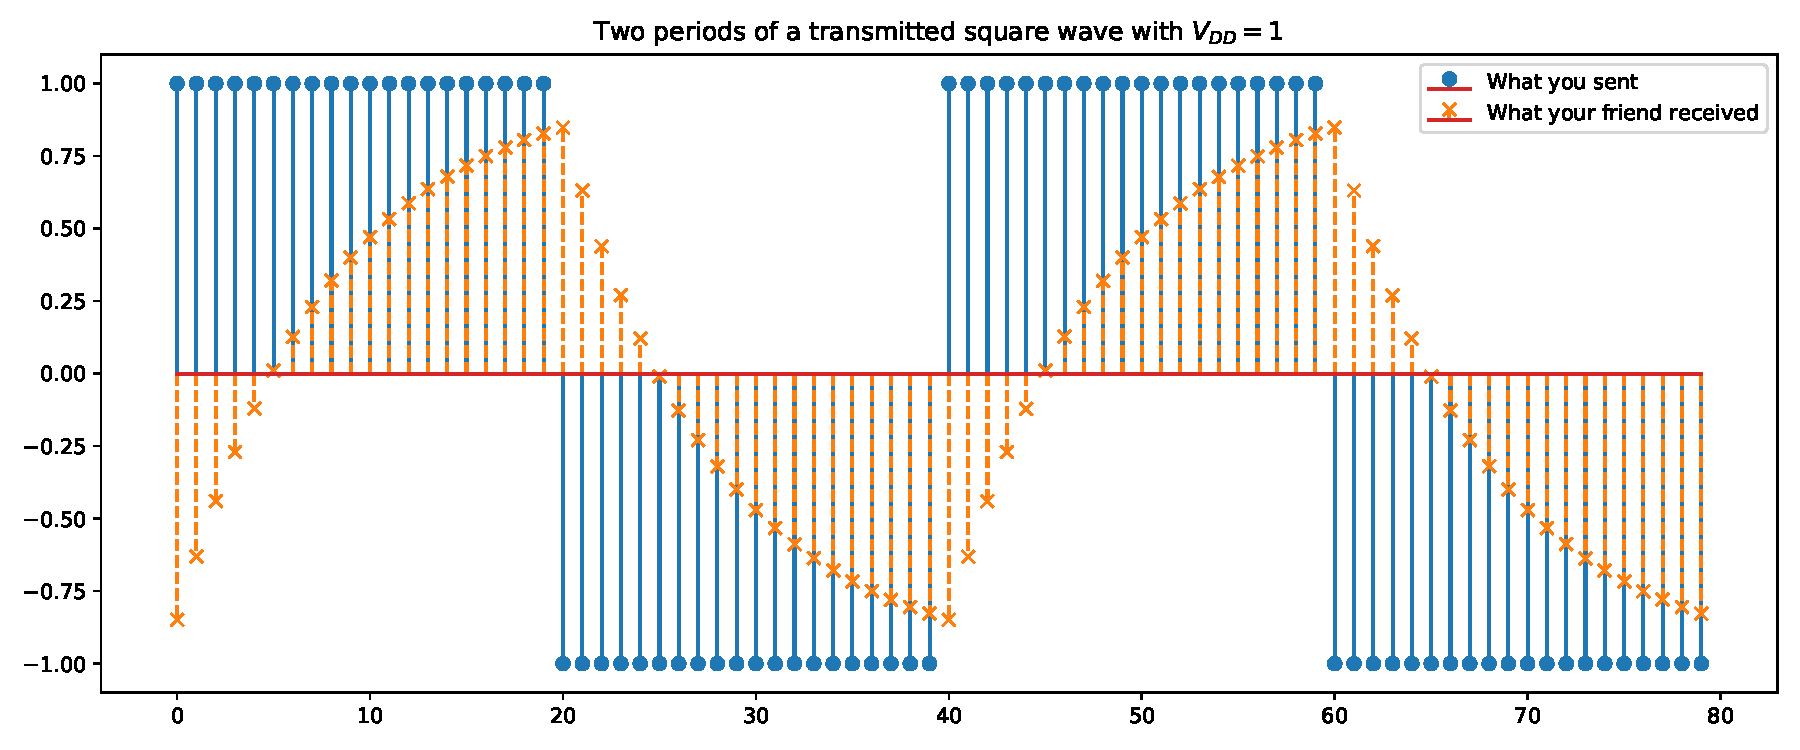
\includegraphics[width=\linewidth]{27-figs/sqwave-lowpassed}
\end{center}
What happened?
The issue is that each wire has a little bit of parasitic resistance \(R\), and there's a parasitic capacitance \(C\) between the two wires.\footnote{Especially if they stay close together.}
The time constant is \(\tau = \frac{1}{2RC}\).

\subsection{Periodic modeling}
We will express a discrete-time model at sampling interval \(T > 0\).
Let \(y[n]\) be the voltage difference at the far end of the cable at time step \(n\), and \(x[n]\) be the voltage difference at the near end.
Then the following recurrence relationship holds:
\begin{align}
  y[n+1]
  &= e^{-T/\tau} y[n] + \del{1 -e^{-T/\tau}} x[n]
  \intertext{Let's choose an even number \(N = M/2\) and send the following square wave:}
  x[n]
  &= \begin{cases}
    1, & n = 0, \ldots, M-1 \quad (\text{mod}\ N)\\
    -1, & n = M, \ldots, N-1 \quad (\text{mod}\ N)
\end{cases}
  \intertext{Therefore we use the state equation to write the following equations describing \(y[1]\) through \(y[N]\):}
  y[1] &= e^{-T/\tau} y[0] + \del{1 - e^{-T/\tau}} x[0] \notag \\
  y[2] &= e^{-T/\tau} y[1] + \del{1 - e^{-T/\tau}} x[1] \notag \\
  \vdots\phantom{[1]} &= \phantom{e^{-T\tau}} \vdots \notag \\
  y[N] &= e^{-T/\tau} y[N - 1] + \del{1 - e^{-T/\tau}} x[N - 1] \notag
  \intertext{Since \(x\) is \(N\)-periodic, so is \(y\) in steady state, so
  \(y[N] = y[0]\) and our last equation is replaced with the following.}
  y[0] &= e^{-T/\tau} y[N - 1] + \del{1 - e^{-T/\tau}} x[N - 1]
  \intertext{
  We can write all \(N\) scalar equations as a single vector equation.
  Treat \(x\) and \(y\) as sample vectors in \(\mathbb{C}^N\).
  Define a circular shift matrix \(S\) such that \((Sy)[n] = y[n+1]\).
  }
  Sy &= e^{-T/\tau} y + \del{1 - e^{-T/\tau}} x \\
  \del{S - e^{-T/\tau} I}y &= \del{1 - e^{-T/\tau}} x \\
  \intertext{We will see later that \(S\)'s eigenvalues are the \(N\)th roots of unity, so \(\del{S - e^{-T/\tau} I}\) is invertible.}
  y &= \del{1 - e^{-T/\tau}}\del{S - e^{-T/\tau} I}^{-1} x.
  \intertext{The matrix \(H \in\mathbb{R}^{n\times n}\) converts a full period of \(x[\cdot]\) to a full period of \(y[\cdot]\). On the near end of the cable \(x\) repeats forever, and on the far end \(Hx\) repeats forever. (Notice that it seems to depend only on things intrinsic to the system itself. It works for any \(x\).)}
  H &= \del{1 - e^{-T/\tau}}\del{S - e^{-T/\tau} I}^{-1}
  \intertext{We will now check that \(H\) makes sense in the cases where \(\tau\) is very small and very large. First, as \(\tau \to 0\), then \(e^{-T/\tau} \to 0\), so}
  H_\text{fast} &= \lim_{\tau \to 0} \del{1 - e^{-T/\tau}}\del{S - e^{-T/\tau} I}^{-1} = S^{-1},
  \intertext{that is, \(y[n] = x[n-1]\). The output waveform is exactly a square wave, reproduced as nearly instantaneously as our sampling interval \(T\) permits. On the other hand}
  H_\text{slow} &=
  \lim_{\tau \to \infty}
  \del{1 - e^{-T/\tau}}\del{S - e^{-T/\tau} I}^{-1} \\
  &= \lim_{\epsilon \to 0} \epsilon \del{S - (1 - \epsilon) I}^{-1}
\end{align}
which is an indeterminate ``0/0'' quotient (numerator becomes zero, and the denominator becomes singular) that I can't find an elementary way to evaluate.\footnote{Let me know if you find one.}

\subsection{In the standard basis}
Let's examine \(H\) by viewing its columns, viz.~the images of the standard basis under \(H\).
Column 0 (the first column) looks like this:
\begin{center}
  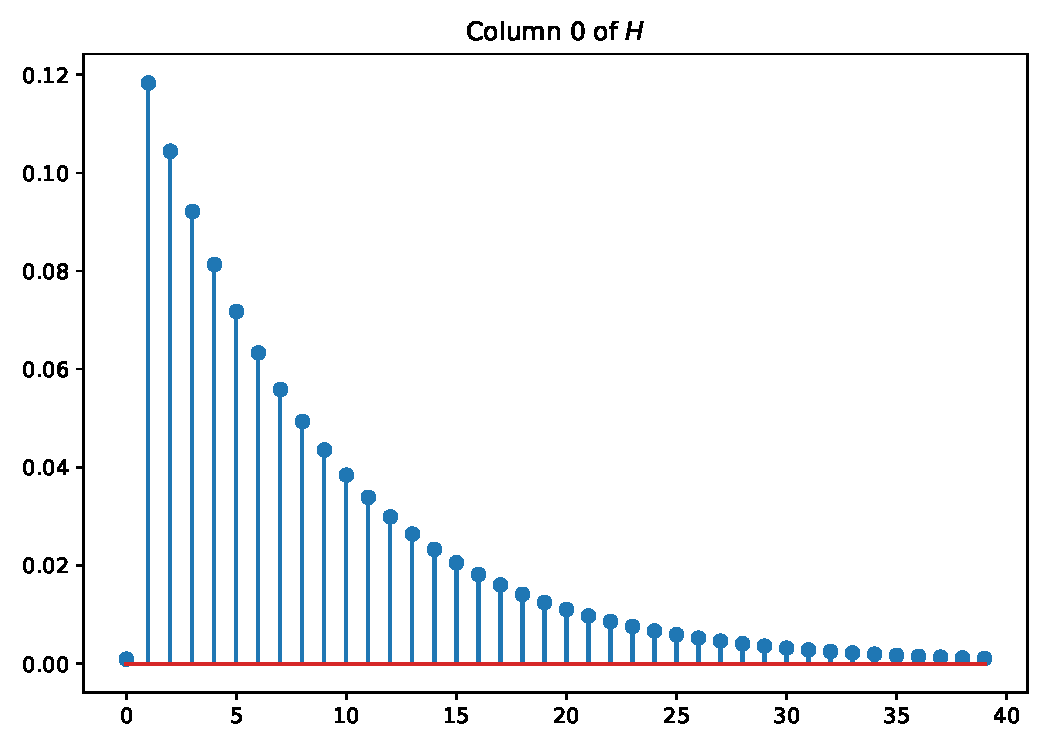
\includegraphics[width=0.618\linewidth]{27-figs/H-0}
\end{center}
and column 1 looks like this:
\begin{center}
  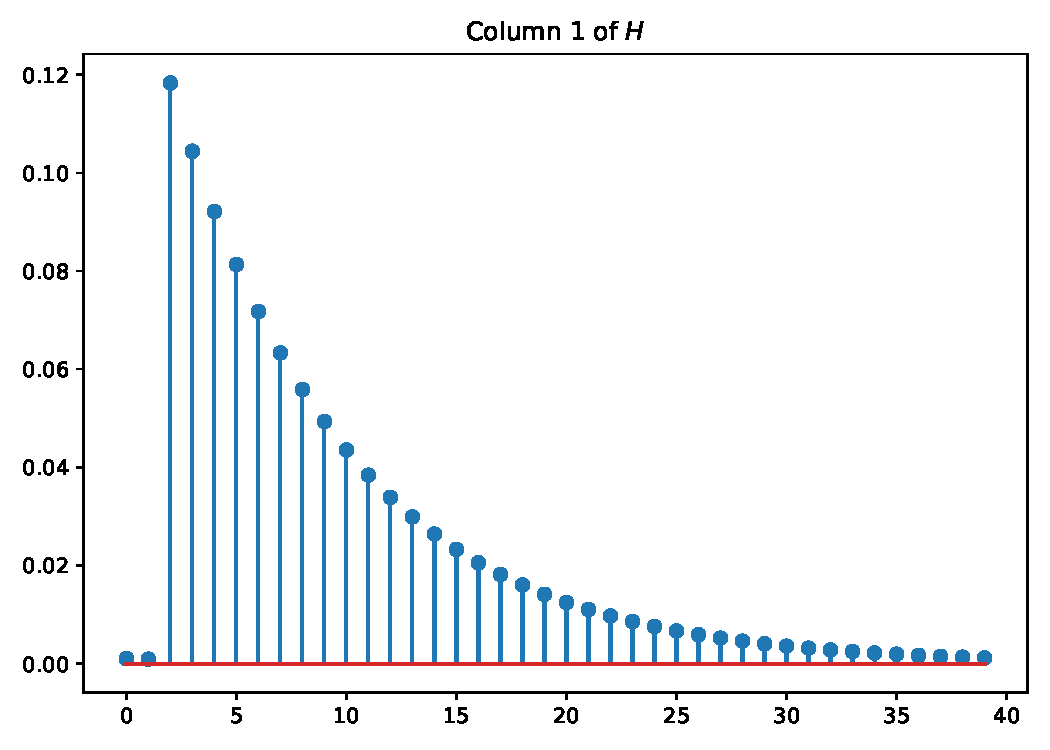
\includegraphics[width=0.618\linewidth]{27-figs/H-1}
\end{center}
You might suspect that column 1 is a right shift\footnote{That is, a right circular shift.} of column 0, and column 2 is a right shift of column 1, and so on.
That would be correct.
% We can prove it like this.
% Because of the circular symmetry of our periodic steady-state equations,
% a shift in the input corresponds to a shift in the output:
% \begin{align}
%   y &= Hx
%   \implies Sy = HSx.
%   % \intertext{We will examine the rela}
% \end{align}

\section{General discrete periodic LTI systems}
Let \(x\in\mathbb{C}^N\) represent a period of input.
Let \(y \in \mathbb{C}^N\) represent a period of input.
A \textbf{linear system} is the relationship\footnote{Lots of \texttt{textbf} ahead! These are definitions!}
\begin{align}
  y &= H x, \quad H \in \mathbb{C}^{N\times N}.
  \intertext{As above, let \(S\) represent a left shift by one sample: \((Sy)[n] = y[n+1]\). If shifts in input correspond to shifts in output, viz.}
  SH &= HS,
  \intertext{the system \(y = Hx\) is called \textbf{time-invariant}.
  Most of our systems from now on with be both linear and time-invariant.
  }
  \intertext{
  When representing periodic signals it is customary to write the standard basis 0-indexed as using the symbol \(\delta_k\) (instead of the ordinary 1-indexed \(e_k\)).}
  \delta_k[n] &=
  \begin{cases}
    1, & n = k\\
    0, & n \neq k
  \end{cases}
  \intertext{\(\delta_i\) is called an \textbf{impulse at time \(i\)}.
  Sometimes \(\delta_0\) is referred to as ``the'' impulse.
  All impulse signals are iterated shifts of \(\delta_0\):}
  \delta_i &= S^{-i} \delta_0
  \intertext{The 0th column of \(H\) is called the \textbf{impulse response} of the linear time-invariant system \(y = Hx\), and it is usually called \(h\).}
  h &= H \delta_0
\end{align}
\section{Convolution: LTI, one impulse at a time}
It is possible to express the LTI system \(y = Hx\) in terms of \(h=H\delta_0\).
Represent \(x\) as a linear combination of standard basis vectors:
\begin{align}
  y &= Hx\\
  &= H\sum_{k = 0}^{N - 1} x[k] \delta_k
  \intertext{Represent each constituent impulse as a shifted \(\delta_0\).}
  &= H\sum_{k = 0}^{N - 1} x[k] \del{S^{-k} \delta_0}\\
  % \intertext{Distribute \(H\) from the left.}
  &= \sum_{k = 0}^{N - 1} x[k] H \del{S^{-k} \delta_0}
  = \sum_{k = 0}^{N - 1} x[k] \del{H S^{-k}} \delta_0
  \intertext{Time-invariance means that \(H\) and \(S\) commute.}
  &= \sum_{k = 0}^{N - 1} x[k] \del{S^{-k} H} \delta_0
  = \sum_{k = 0}^{N - 1} x[k] S^{-k} \del{H\delta_0}\\
  &= \sum_{k = 0}^{N - 1} x[k] S^{-k} h
  \intertext{When \(x = \delta_n\), this equation verifies our earlier observation that all columns of \(H\) are right circular shifts of \(h\). Now let's make a formula for sample \(n\) of the output.}
  y[n] &= \sum_{k = 0}^{N - 1} x[k] \del{S^{-k} h}[n] \\
  &= \sum_{k = 0}^{N - 1} x[k] h[n -k]
  % \intertext{}
\end{align}
This formula is called the \textbf{circular convolution} of \(x\) with \(h\).

\chapter{Convolution and the DFT}
The DFT diagonalizes convolutions.
Throughout, let \(S \in\mathbb{C}^N\) be the left circular shift matrix defined by
% \begin{align}
  \((Sx)[n] = x[n+1]\),
  % \intertext{
  where circular indexing is understood.
% \end{align}

% \section{Eigendecomposition of circular shift}
\begin{lemma}[Eigendecomposition of circular shift]
  The eigenvectors of \(S\) are the DFT basis vectors, and that the eigenvalues are the roots of unity.\footnote{We could just verify this directly, but I find that diagonalizing \(S\) helps to clarify the magic surrounding the DFT basis.}
\end{lemma}
\begin{proof}
To show this, suppose we have an eigenvalue-eigenvector pair
\begin{align}
  Sv &= \lambda v.
  \intertext{Multiplying through by \(S^{N-1}\),}
  S^N v &= \lambda S^{N - 1} v = \lambda^2 S^{N-2} v = \ldots = \lambda^N v.
  \intertext{On the left, \(S^N = I\) as \(N\) rotations amount to a revolution.}
  v &= \lambda^N v \\
  \del{\lambda^N - 1} v &= 0
  \intertext{As \(v\) is nonzero by virtue of being an eigenvector, by the zero product property,}
  \lambda^N &= 1\\
  \lambda &= \omega_N^0, \omega_N^1, \ldots, \omega_N^{N - 1}
  \intertext{Let's solve for \(u_k\), the eigenvector corresponding to \(\omega^k\).}
  S u_k &= \omega^k u_k \\
  % \intertext{At position \(n + }
  u_k[n + 1] &= \omega^k u_k[n]
  % \intertext{This so}
\end{align}
This shows that \(u_k\) consists of consecutive powers of \(\omega^k\).
Normalizing by \(\del{\sqrt{N}}^{-1}\) we have the DFT basis.
\end{proof}

% The eigenvalues of \(S\) are the \(N\)th roots of unity are the essence of all things \(N\)-periodic.

% \section{Interlude: matrix polynomials}
A \textbf{polynomial} in the indeterminate \(z\) is an expression of the form
\(p(z) = \sum_{k = 0}^{d} p_k z^k\), where \(d \geq 0\).
When \(p(z)\) is evaluated at a matrix \(A\), we use \(A^0 = I\).
\begin{lemma}[Eigendecomposition of a matrix polynomial]
  % \tag{lemma:matpol}
  Let \(A \in\mathbb{C}^{n\times n}\), and let \(p(z)\) be a polynomial in the indeterminate \(z\).
  Then if \(Av = \lambda v\) is an eigenvalue-eigenvector pair,
  then \(p(A) v = p(\lambda) v\).
\end{lemma}
\begin{proof}
  Let \(d\) be the degree of \(p\).
  \begin{align}
    p(A) v &= \sum_{k=0}^{d} p_k A^k v\\
    \intertext{It can be shown by induction on \(k\) that \(A^k v = \lambda^k\)v.}
    p(A) v &= \sum_{k=0}^{d} p_k \lambda^k v \\
    &= \del{\sum_{k=0}^{d} p_k \lambda^k} v\\
    &= p(\lambda) v
  \end{align}
  Therefore \(p(A)\) has the same eigenvectors as \(A\), but the eigenvalues are \(p(\lambda)\) for each eigenvalue \(\lambda\) of \(A\).
\end{proof}

\subsection{Example: Cayley-Hamilton theorem}
We can use calculus to show that if \(\chi\) is the characteristic polynomial of \(A\in\mathbb{C}^{n\times n}\), then \(\chi(A) = 0\).
First, if \(A\) is diagonalizable, then for every eigenvalue-eigenvector pair
\(A v = \lambda v\), we have \(\chi(A) v = \chi(\lambda) v = 0v\).
The matrix \(\chi(A)\) annihilates the eigenvectors of \(A\), which are a basis for \(\mathbb{C}^N\). Therefore \(\chi(A) = 0\).

If \(A\) is not diagonalizable, then let \(A = U M U^*\), where \(M\) is upper triangular and \(U\) is unitary.
Let \(D\) be a diagonal matrix such that \((M+\epsilon D)\) has no repeated diagonal elements for all sufficiently small \(\epsilon > 0\).
Let \(A_\epsilon = U\del{M + \epsilon}U^*\).
Then \(\chi_A(A) = \lim_{\epsilon \to 0} \chi_{A_\epsilon}(A_\epsilon)\).
For all \(\epsilon > 0\), \(A_\epsilon\) is diagonalizable and therefore vanishes under its own characteristic polynomial.
As polynomial functions are continuous, therefore \(\chi_A(A) =0 \).
% For every \(\epi

\subsection{Example: heat equation on a ring}
Let \(x[t] \in \mathbb{R}^N\) represent the temperatures of a solid ring, sampled at evenly spaced intervals.
According to the heat equation\footnote{Solved by Fourier using a continuous-time analog of the DFT.}, \(x\) evolves according to the following law:
\begin{align}
  x[t+1] &= A x[t], \quad \text{where} \\
  A &= \frac{1}{4}(2I + S + S^{N-1}).
  \intertext{\(A\) may be written as \(p(S)\), where \(p\) is the following polynomial:}
  p(z) &= \frac{1}{4}(2 + z + z^{N-1})
  \intertext{Therefore the eigenvectors of \(A\) are the DFT basis vectors, and the eigenvalues of \(A\) are}
  p(\omega_N^k)
  &= \frac{1}{4}(2 + \omega_N^k + \omega_N^{-k}) = \frac{1}{2}\del{1 + \cos{2\pi k/N}},
\end{align}
and this system is marginally stable.


\section{\(H\) is polynomial in \(S\), and a lot of conclusions}
If \(y = Hx\) for \(x,y \in\mathbb{C}^N\) is a linear time-invariant system with impulse response \(h\),
 then \(H\) is constant along stripes parallel to the diagonal.
 Decomposing \(H\) into its \(N\) stripes,
\begin{align}
  H &= \sum_{k=0}^{N-1} h[k] S^{-k}
  \intertext{Multiplying by \(S^N = I\),}
   &= \sum_{k=0}^{N-1} h[k] S^{N -k}\\
  &= \sum_{k=0}^{N-1} h[k] S^{N -k}\\
  &= p(S),\ \text{where}\
  \ p(z) = \sum_{k=0}^{N-1} h[k] z^{N- k}.\\
  \intertext{Therefore \(H\), being a polynomial in \(S\), has the same eigenvectors as \(S\). The DFT basis vector \(u_k\) satisfies \(Su_k = \omega_N^k u_k\), so it is also an eigenvector of \(H\) with eigenvalue \(p(\omega_N^k)\):}
  H u_k &= p(\omega^k) u_k
  \intertext{Let's find out what our eigenvalue \(p(\omega^k)\) is.}
  p(\omega^k)
  &= \sum_{\ell=0}^{N-1} h[\ell] \omega^{k(N- \ell)}
  \intertext{It's row \(k\) of the DFT analysis equation! Using the DFT}
  g &= Fh,\\
  \intertext{we have}
  p(\omega^k) &= \sqrt{N} g[k].
  \intertext{Therefore \(H\) has the following eigendecomposition:}
  H
  &= F^*
   G
  F =
  F^* \operatorname{diag}\{g\} F\\
  &=
  F^*
  \begin{pmatrix}
    \sqrt{N} g[0]      &   &    \\
     & \sqrt{N}  g[1] \\
     &                 & \ddots &\\
     &                &         & \sqrt{N} g[N-1]
  \end{pmatrix}
  F.
  \intertext{In the DFT basis, time domain convolution is represented as a pointwise multiplication (using the symbol \(\odot\)).}
  Fy &= \del{\sqrt{N} Fh} \odot Fx
\end{align}
Efficient algorithms for DFT and inverse DFTs can take advantage of the fact that \(F\) and \(F^*\) are symmetric matrices.
They run as fast as an efficient sorting algorithm.

\section{Square wave transmission, revisited}
\subsection{An indeterminate matrix limit}
We derived that the convolution matrix of a transmission line with time constant \(\tau\) is
\begin{align}
  H &= \del{1 - e^{-T/\tau}} \del{S - e^{-T/\tau} I} ^{-1}.
  \intertext{We showed that as \(\tau\to0\), \(H\to S^{-1}\), a one-sample delay.
  As \(\tau\to \infty\), \(\del{1 - e^{-T/\tau}} \to 0\), we have a ``0/0'' limit.}
  H_\text{slow}
  &= \lim_{\epsilon \to 0} \epsilon \del{S - \del{1-\epsilon} I}^{-1}
  \intertext{Diagonalize \(S\) as \(S = F^* \Omega F\), where \(\Omega = \operatorname{diag}\left\{\omega_N^0, \omega_N^1, \ldots, \omega_N^{N-1}\right\}\).}
  &= \lim_{\epsilon \to 0} \epsilon \del{F^*\Omega F - \del{1-\epsilon} I}^{-1}\\
  &= \lim_{\epsilon \to 0}
  \epsilon \del{F^*\del{\Omega  - \del{1-\epsilon} I}F}^{-1} \\
  &= \lim_{\epsilon \to 0}
  F^*\del{\frac{\Omega  - \del{1-\epsilon} I}{\epsilon}}^{-1}F \\
  &= \lim_{\epsilon \to 0}
  F^*
  \operatorname{diag}\left\{
    \frac{\epsilon}{\omega_N^0 - 1 + \epsilon},
    \frac{\epsilon}{\omega_N^1 - 1 + \epsilon}, \ldots,
    \frac{\epsilon}{\omega_N^{N-1} - 1 + \epsilon}
  \right\}
  F \\
  &= \lim_{\epsilon \to 0}
  F^*
  \operatorname{diag}\left\{
    \frac{\epsilon}{\epsilon},
    \frac{\epsilon}{\del{\text{nonzero}}}, \ldots,
    \frac{\epsilon}{\del{\text{nonzero}}}
  \right\}
  F \\
  &=
  F^*
  \operatorname{diag}\left\{1, 0, \ldots, 0 \right\}
  F \\
  &=
  \frac{1}{N}
  \begin{pmatrix}
    1 & \cdots & 1 \\
    \vdots & \ddots & \vdots \\
    1 & \cdots & 1 \\
  \end{pmatrix}
\end{align}
As our transmission line becomes infinitely slow, eventually it becomes impossible to move the output at all, and all AC signals are shorted through the parasitic shunt capacitor.
Only the DC component of the input passes.

\subsection{Input, transfer function, output}

\begin{figure}
  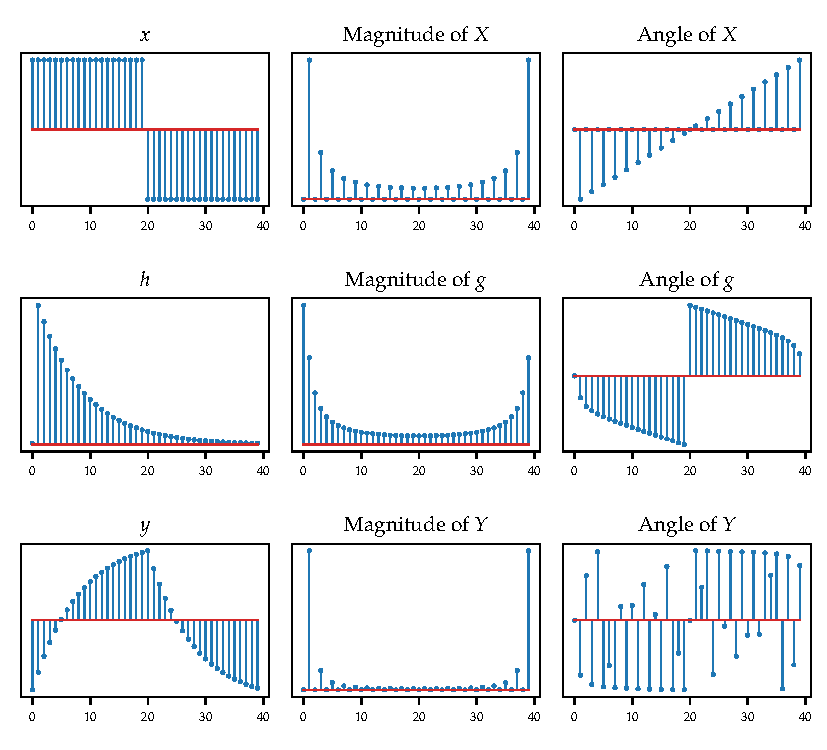
\includegraphics{27-figs/inHout}
  \caption{Input, impulse response, and output in time and frequency domain.}
  \label{fig:lec27-inHout}
\end{figure}
The left column of Figure~\ref{fig:lec27-inHout} shows:
\begin{itemize}
  \item \(x\), the square wave on the near end of the transmission line;
  \item \(h\), the impulse response of the transmission line; and
  \item \(y\), the output on the far end of the transmission line.
\end{itemize}
We showed that \(y\) is the convolution of \(x\) with \(h\).

The center and right columns of Figure~\ref{fig:lec27-inHout} show:
\begin{itemize}
  \item \(X= Fx\), the ``phasor'' representation of \(x\) in the DFT basis (note that \(x\) has only odd frequencies);
  \item \(g = Fx\), the ``transfer function'' representation of \(h\) in the DFT basis (can you tell that \(g\) is a low-pass filter?); and
  \item \(Y = \sqrt{N} g \odot X\), the ``phasor'' representation of \(y\) in the DFT basis. (When eyeballing \(g \odot X\), remember that magnitudes multiply and phases add.)\footnote{The phase of \(Y\) is crazy; don't think too hard about what it means.}
\end{itemize}

\subsection{Equalization using DFT}
\begin{figure}
  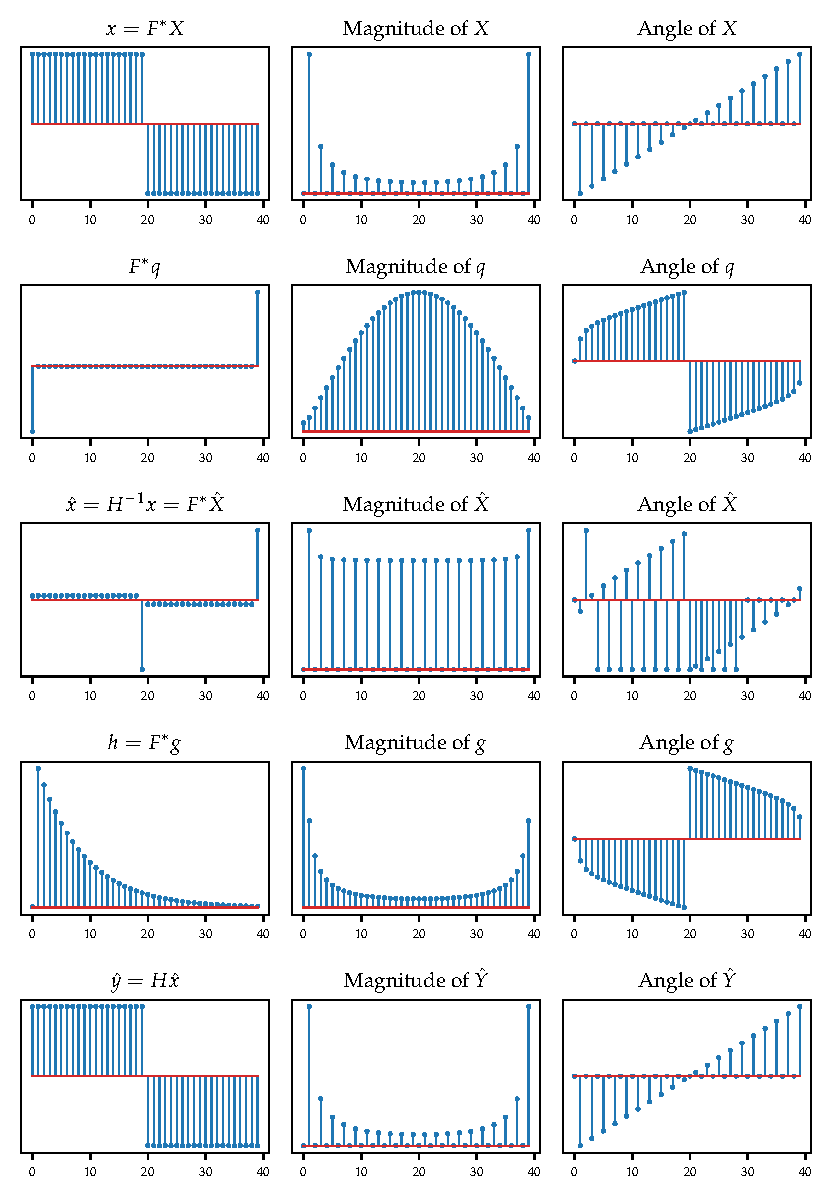
\includegraphics{27-figs/eq}
  \caption{Input, impulse response, and output in time and frequency domain.}
  \label{fig:lec27-eq}
\end{figure}

The transmission equation
\begin{align}
  y &= Hx \\
  \intertext{has the frequency domain representation}
  Y &= \sqrt{N} g \odot X,
  \intertext{where \(Y = Fy\), \(g = Fh\), and \(X = Fx\). To achieve a square wave output, we can cancel \(\sqrt{N}g\) by pre-dividing by \(\sqrt{N}g\). That is, define a frequency response \(q\) by}
  q[n] &= \frac{1}{\sqrt{N}g[n]},
  \intertext{then define our pre-equalized input \(\hat X\) in frequency domain by}
  \hat X &= q[n] \odot X,
  \intertext{resulting in}
  \hat Y &= \sqrt{N} g \odot \hat X = \sqrt{N} g\odot \del{q \odot X} = X
\end{align}
Therefore \(F^* \hat X\) is what you should send in order to make sure your friend across the lab receives the square wave \(X\).
Figure~\ref{fig:lec27-eq} shows the pre-equalized input, equalization filter, equalized input, transmission filter, and output.
Observe that equalization is the inverse of transmission.


\end{document}
